\documentclass[12pt]{article}
\usepackage{graphicx}
\usepackage[T1]{fontenc}
\usepackage[italian]{babel}
\usepackage{tocloft}
\usepackage{subcaption}
\usepackage{caption}
\usepackage{hyperref}
\usepackage{booktabs}
\usepackage{listings}
\usepackage{wrapfig}
\usepackage{pdfpages}
\usepackage{pdflscape}
\usepackage{scrlayer}
\usepackage{scrhack}
\renewcommand{\cftsecdotsep}{2}
\renewcommand{\cftsubsecdotsep}{2}
\renewcommand*{\thefootnote}{(\arabic{footnote})}
\hypersetup{
    colorlinks,
    citecolor=black,
    filecolor=black,
    linkcolor=black,
    urlcolor=black
}
\DeclareNewLayer[
background,
textarea,
addwidth=\footskip,
addwidth=\footheight,
contents=\hfill
\rotatebox{90}{\parbox{\layerheight}{\centering\pagemark}}]{lscape.foot}
\DeclareNewPageStyleByLayers{lscape}{lscape.foot}
\graphicspath{{images/}}
\begin{document}
\begin{titlepage}
    \centering
    
\includegraphics[width=100pt]{logo-polimi-new}\par\vspace{1cm}
    {\scshape\LARGE Politecnico di Milano \par}
    \vspace{1cm}
    {\scshape\Large Progetto Finale di Reti Logiche \par}
    \vspace{1.5cm}
    {\huge\bfseries Codifica Working Zone\par}
    \vspace{2cm}
    {\Large \textit{Nicolò Sonnino}\par}
    \vfill
    supervisore\par
    Prof.\ Gianluca \textsc{Palermo}
    \vfill
    {\large \today \par}
\end{titlepage}
\tableofcontents
\newpage
\section{Specifiche}
\subsection{Descrizione}
Il progetto ha come scopo la realizzazione della codifica \textbf{working zone}, questa strategia viene utilizzata sopratutto nello sviluppo di microprocessori.\newline
Il consumo di energia dei pin è una parte integrante nella loro progettazione, per ridurlo, si suppone, che determinati programmi favoriscano poche zone all'interno del loro spazio di memoria in ogni istante.\newline
Quindi vengono identificate tali zone e con un riferimento dell'indirizzo scelto viene inviato anche un offset codificato "one-hot" per trovare la sua posizione rispetto all'indirizzo base della working zone.\par
\subsection{WZE (Working Zone Encoding)}
Il progetto presenta una memoria RAM da 65536 indirizzi con valore base di 8 bit per ogni cella di memoria; di questi i primi otto sono riempiti con indirizzi base, mentre il nono contiene il valore da codificare e il decimo è quello riservato alla scrittura del risultato codificato.\newline
A questo punto abbiamo due possibili casi: il valore rientra in una delle working zones, oppure non appartiene a nessuno dei sette indirizzi; nel primo caso si identifica la working zone (WZ\_NUM) e l'offset rispetto ad essa (WZ\_OFFSET), si pone WZ\_BIT\(=\) 1 e si scrive nell'indirizzo di posizione 9 WZ\_BIT \& WZ\_NUM \& WZ\_OFFSET\footnote[1]{\& simbolo di concatenazione}, mentre nel secondo caso viene posto WZ\_BIT\(=\) 0, il valore (ADDR) viene salvato e l'output risulta WZ\_BIT \& ADDR.\newline
L'offset \textbf{one-hot} associa all'unico 1 il valore da rappresentare nel seguente modo:
\begin{itemize}
    \item WZ\_OFFSET \(=\) 0 \(=>\) \textbf{"0001"}
    \item WZ\_OFFSET \(=\) 1 \(=>\) \textbf{"0010"}
    \item WZ\_OFFSET \(=\) 2 \(=>\) \textbf{"0100"}
    \item WZ\_OFFSET \(=\) 3 \(=>\) \textbf{"1000"}
\end{itemize}
\newpage
\subsection{Esempi}
\begin{figure}[!htb]
    \centering
    \begin{minipage}[b]{1\textwidth}
        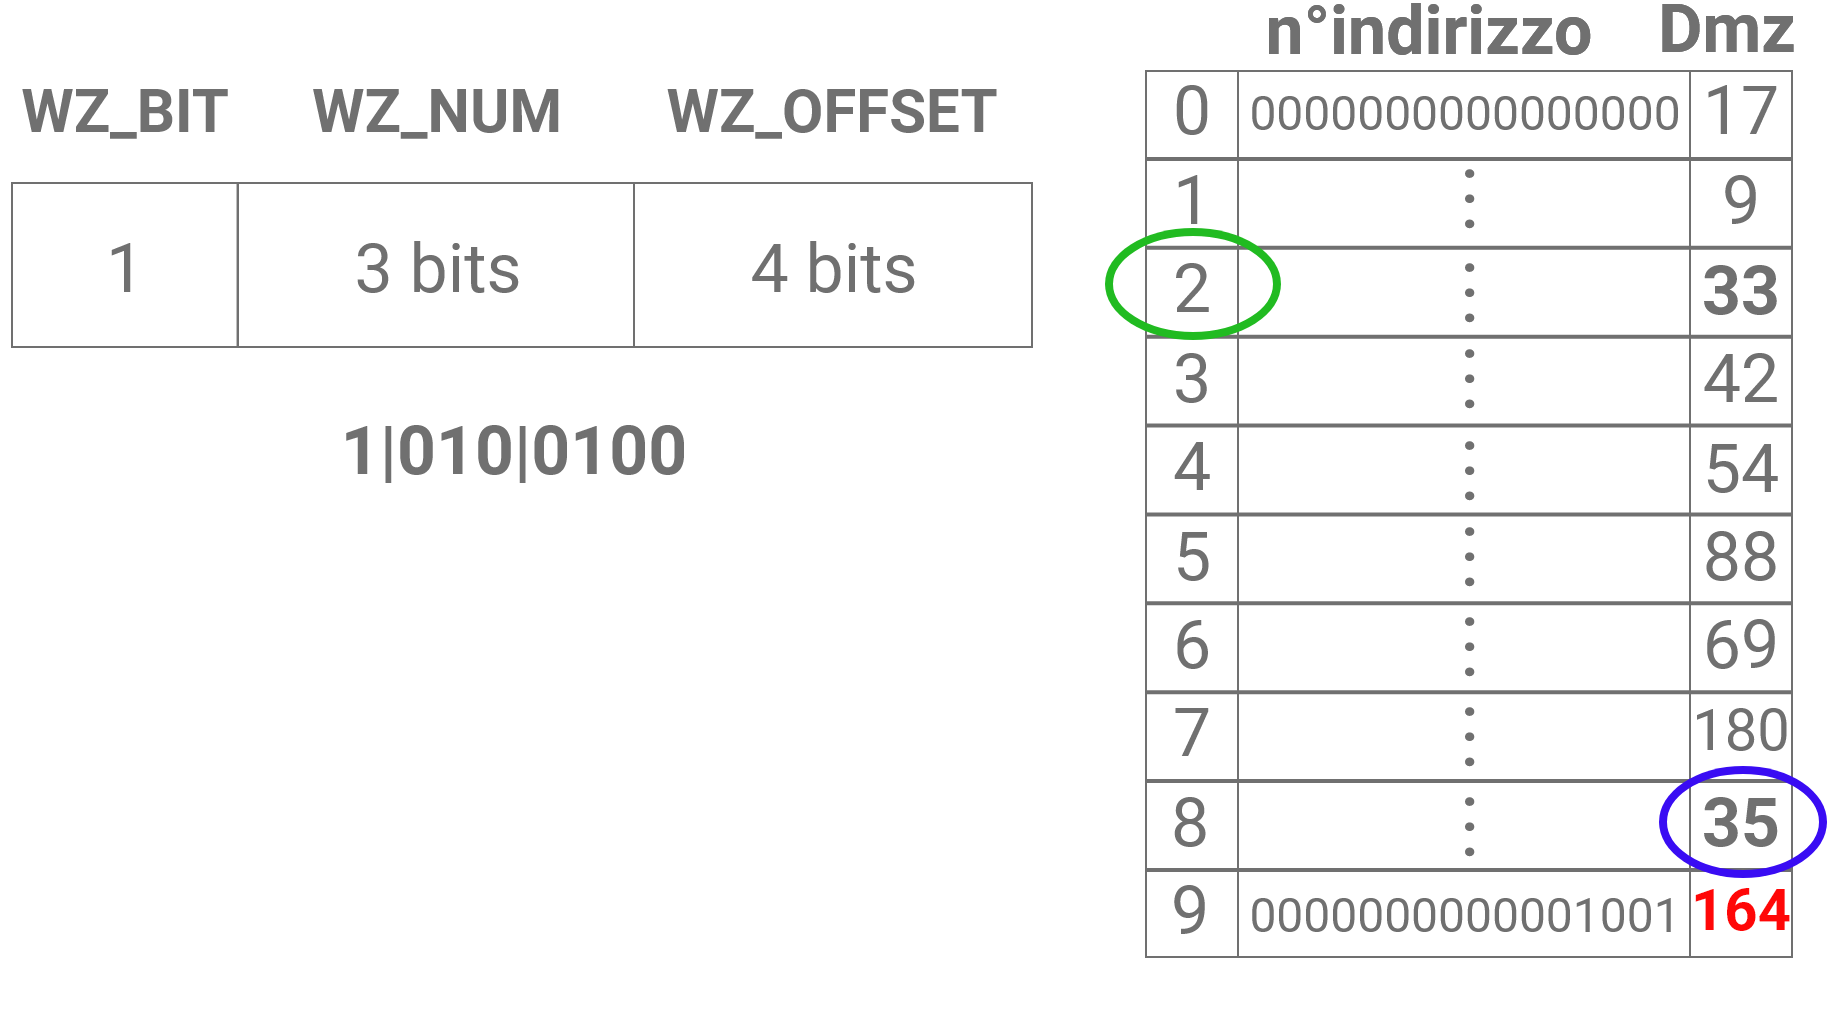
\includegraphics[scale=0.21]{WZ_IN.png}
        \captionsetup{justification=centering}
        \caption{Valore contenuto in posizione 2}\label{WZ_IN}
    \end{minipage}
    \hfill
    \vspace{0.2cm}
    \begin{minipage}[b]{1\textwidth}
        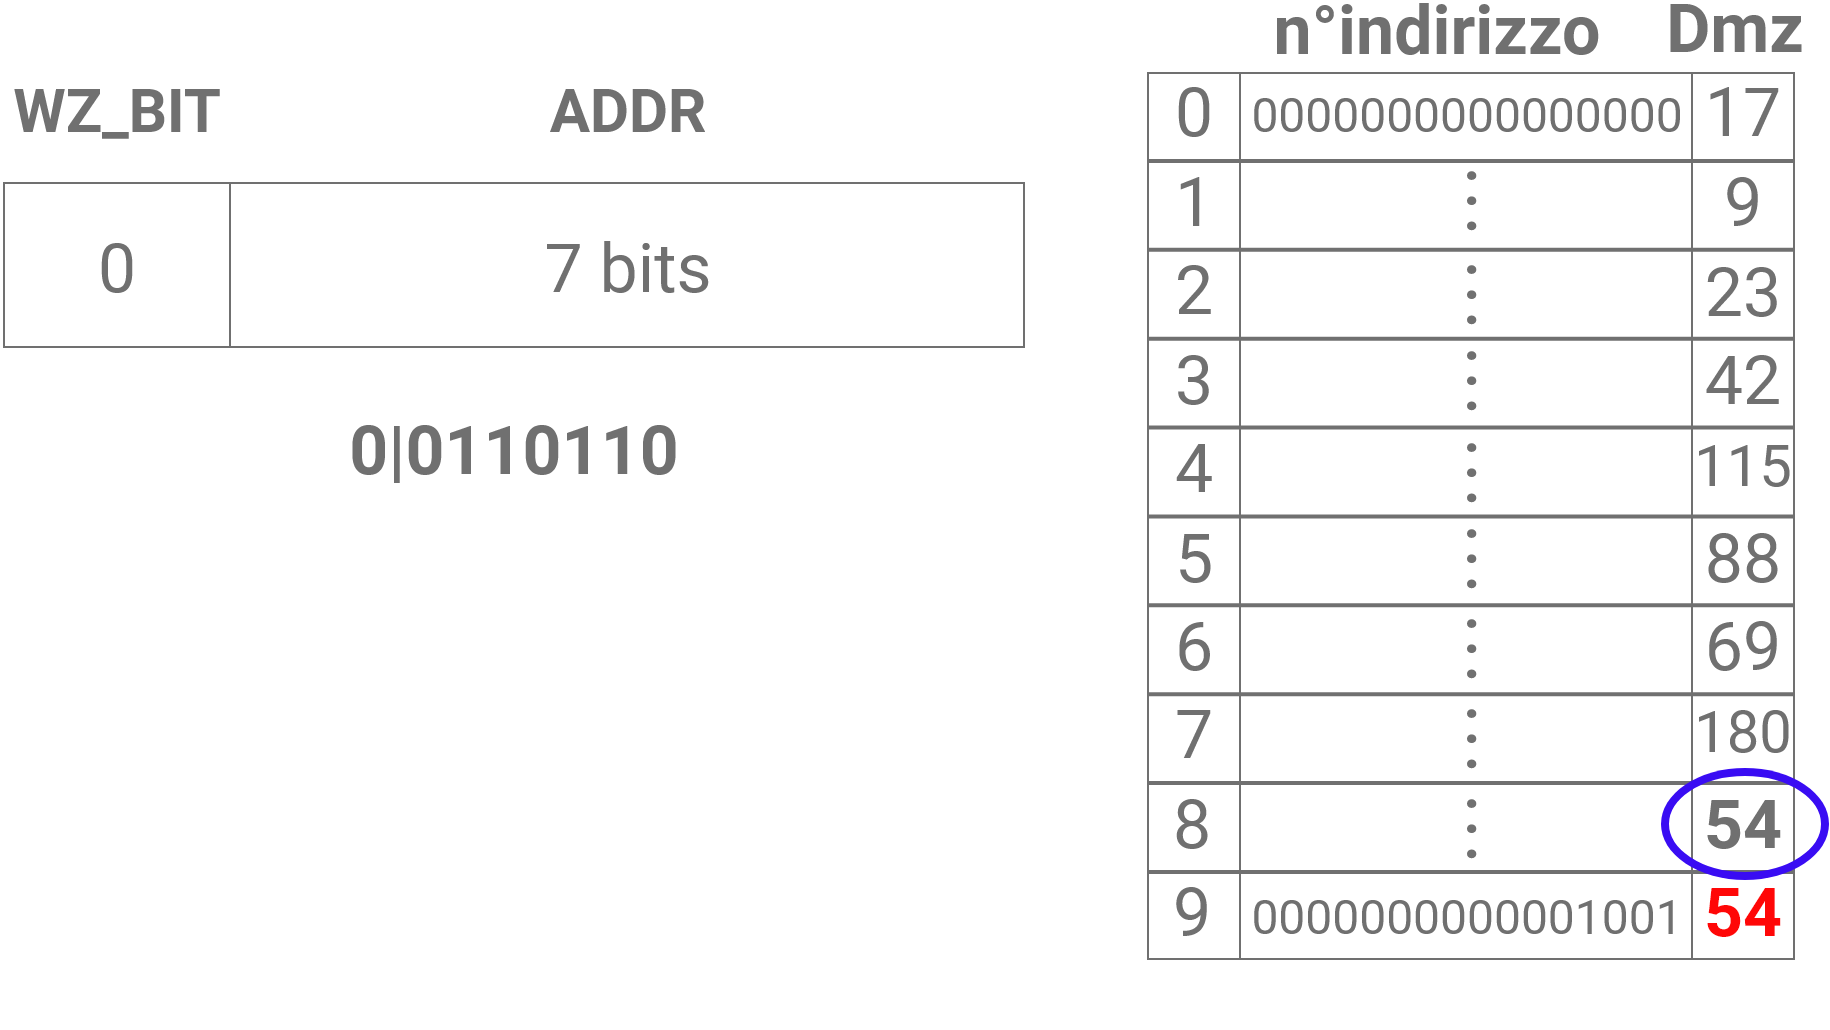
\includegraphics[scale=0.21]{WZ_OUT.png}
        \captionsetup{justification=centering}
        \caption{Valore non contenuto in nessuna working zone}\label{WZ_OUT}
    \end{minipage}
\end{figure}
\newpage
\section{Architettura}
Di seguito viene mostrata la FSM (Final State Machine) in versione semplificata, sono omessi tutti gli anelli che da qualsiasi stato tornano a \textbf{reset} quando \textbf{i\_rst\(=\)'1'}.\newline
\\Descrizione di ogni stato:
\begin{itemize}
    \parbox[t]{\dimexpr\textwidth-\leftmargin}{%
    \vspace{-2.5mm}
    \begin{wrapfigure}[19]{r}{0.45\textwidth}
        \centering
        \vspace{-\baselineskip}
        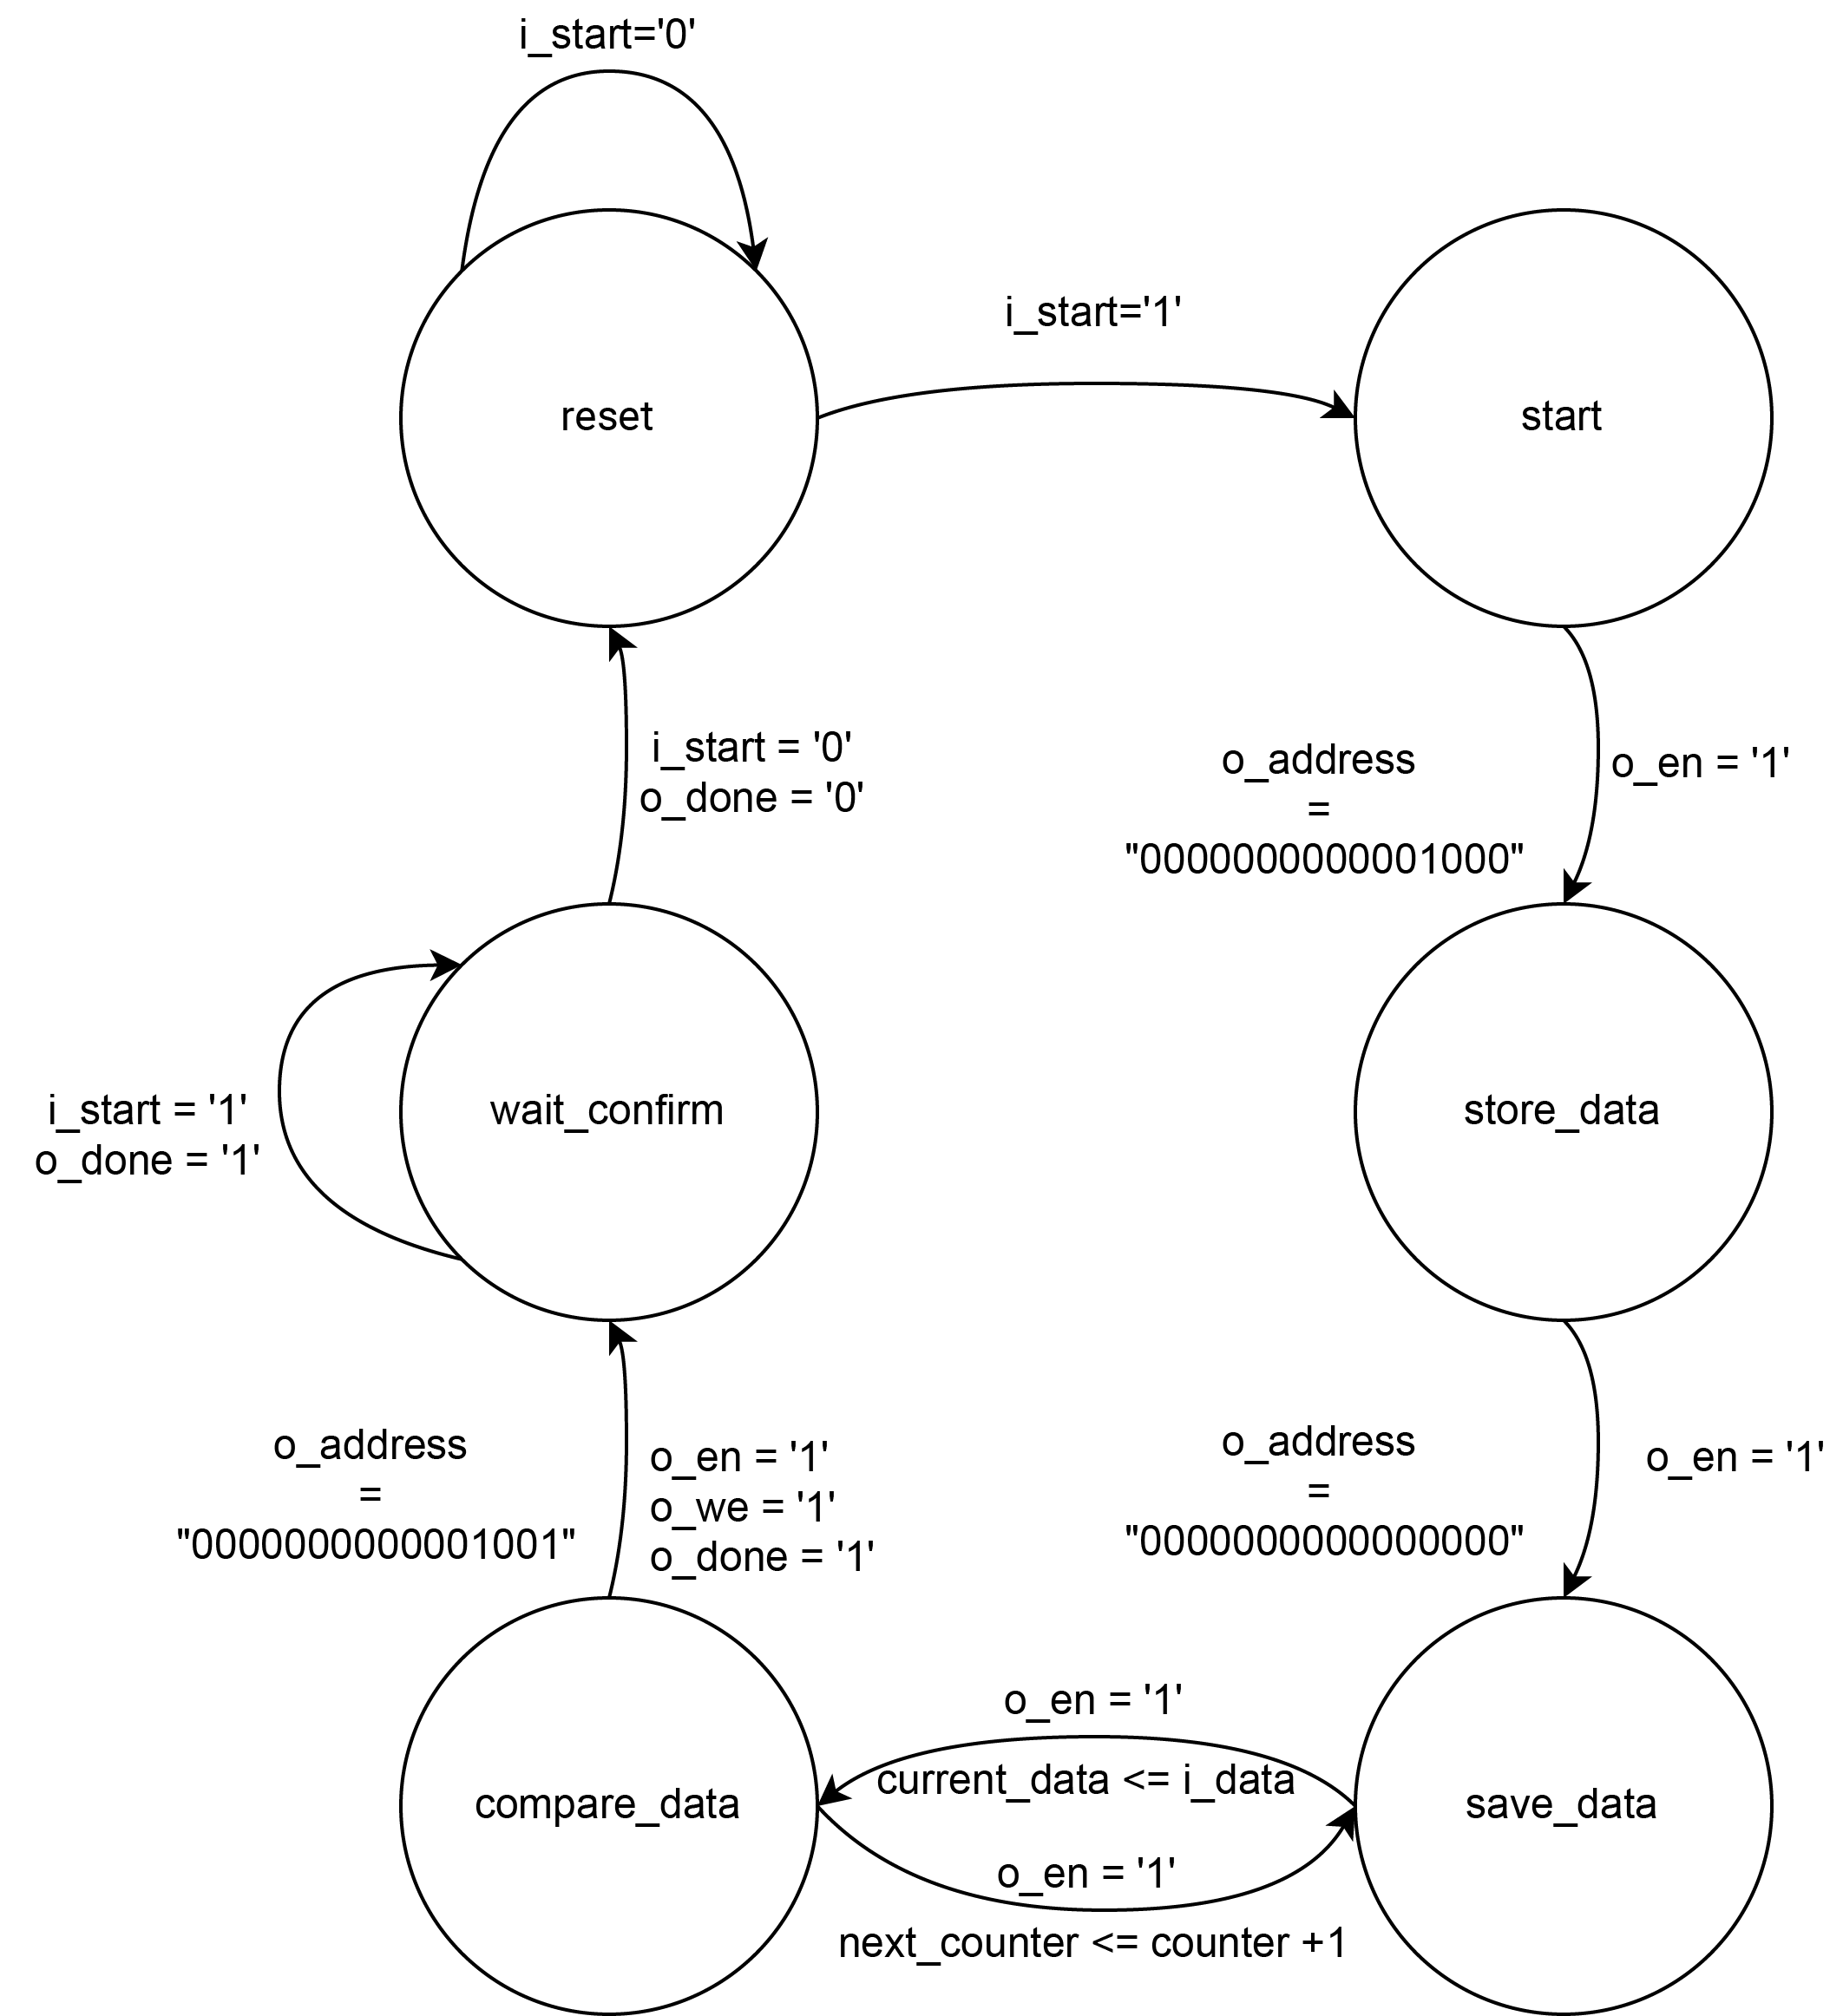
\includegraphics[width=0.65\textwidth]{FSM.png}
    \end{wrapfigure}
    \item \textbf{reset}: stato di inizializzazione, se il segnale \textbf{i\_rst} viene alzato si ritorna a questo stato. Fintanto che \textbf{i\_start} rimane basso si ritorna a reset, se viene alzato si passa a start.
    \item \textbf{start}: stato di preparazione, i segnali \textbf{o\_we, wz\_bit} vengono abbassati, l'\textbf{offset} viene posto a 0000; per permettere la lettura dell'indirizzo in posizione 8, \textbf{o\_en} viene alzato a 1 e si assegna 0000000000001000 a \textbf{o\_address}.
    \item \textbf{store\_data}: stato di memorizzazione del valore da codificare, \textbf{i\_data} letto precedentemente viene salvato nel registro \textbf{data} e viene inizializzato il valore \textbf{next\_counter}, responsabile di iterare gli indirizzi di memoria.
          }
    \item \textbf{save\_data}: stato di salvataggio, il valore di \textbf{i\_data} viene salvato per essere utilizzato per confrontarlo successivamente.
    \item \textbf{compare\_data}: stato di confronto dei valori, attraverso un contatore interno allo stato si confronta il valore di \textbf{data} con \textbf{current\_data} con sommato il contatore; se risultano uguali viene abilitata la scrittura tramite l'assegnazione di \textbf{o\_en} e \textbf{o\_we} a 1 e \textbf{o\_address} viene posto a 9, infine \textbf{o\_data} viene codificato come discusso nelle specifiche e \textbf{o\_done} viene alzato a 1. Nel caso in cui non appartenga alla working zone, se non è al ottavo indirizzo, il contatore viene incrementato e si ritorna allo stato precedente, altrimenti viene abilitata la scrittura  del valore codificato  e si alza \textbf{o\_done}.
    \item \textbf{wait\_confirm}: stato di attesa, se allo stato precendente è stato alzato \textbf{o\_done} si arriva a quest'ultimo; vengono quindi azzerati i segnali di scrittura e lettura, \textbf{o\_done} rimane alzato fino a quando non viene ricevuto un segnale \textbf{i\_start} = 0 e allora in quel caso \textbf{o\_done} viene abbassato e si ritorna a reset.
\end{itemize}
\section{Risultati Sperimentali}
\subsection{Sintesi}
Il progetto è stato testato sulla versione di \textbf{Vivado 2016.4}, utilizzando come FPGA target \textbf{xc7a200tfbg484-1}, e ha generato il seguente report di sintesi:\\
\\
\begin{tabular}{lcccc}
    \toprule
    Site Type                   & Used & Fixed & Available & Util\% \\
    \midrule
    Slice LUTs*                 & 46   & 0     & 134600    & 0.03   \\
    \quad LUT as Logic          & 46   & 0     & 134600    & 0.03   \\
    \quad LUT as Memory         & 0    & 0     & 46200     & 0.00   \\
    Slice Registers             & 19   & 0     & 269200    & <0.01  \\
    \quad Register as Flip Flop & 5    & 0     & 269200    & <0.01  \\
    \quad Register as Latch     & 14   & 0     & 269200    & <0.01  \\
    F7 Muxes                    & 0    & 0     & 67300     & 0.00   \\
    F8 Muxes                    & 0    & 0     & 33650     & 0.00   \\
    \bottomrule
\end{tabular}
\\
\\Per gli stati e il consumo invece:\newline\newline
\begin{tabular}[t]{lcc}
    \toprule
    State         & New Enc. & Previous Enc. \\
    \midrule
    reset         & 000      & 000           \\
    start         & 001      & 001           \\
    store\_data   & 010      & 010           \\
    save\_data    & 011      & 011           \\
    compare\_data & 100      & 100           \\
    wait\_confirm & 101      & 101           \\
    \bottomrule
\end{tabular}
\quad
\begin{tabular}[t]{llc}
    \toprule
    Type          & Power   & Util\% \\
    \midrule
    Signals       & 0.448 W & 16\%   \\
    Logic         & 0.285 W & 10\%   \\
    I/O           & 2.059 W & 74\%   \\
    Device Static & 0.142 W & 5\%    \\
    \bottomrule
\end{tabular}
\subsection{Simulation}
\vspace{-0.2 cm}
\begin{figure}[!htb]
    \begin{center}
        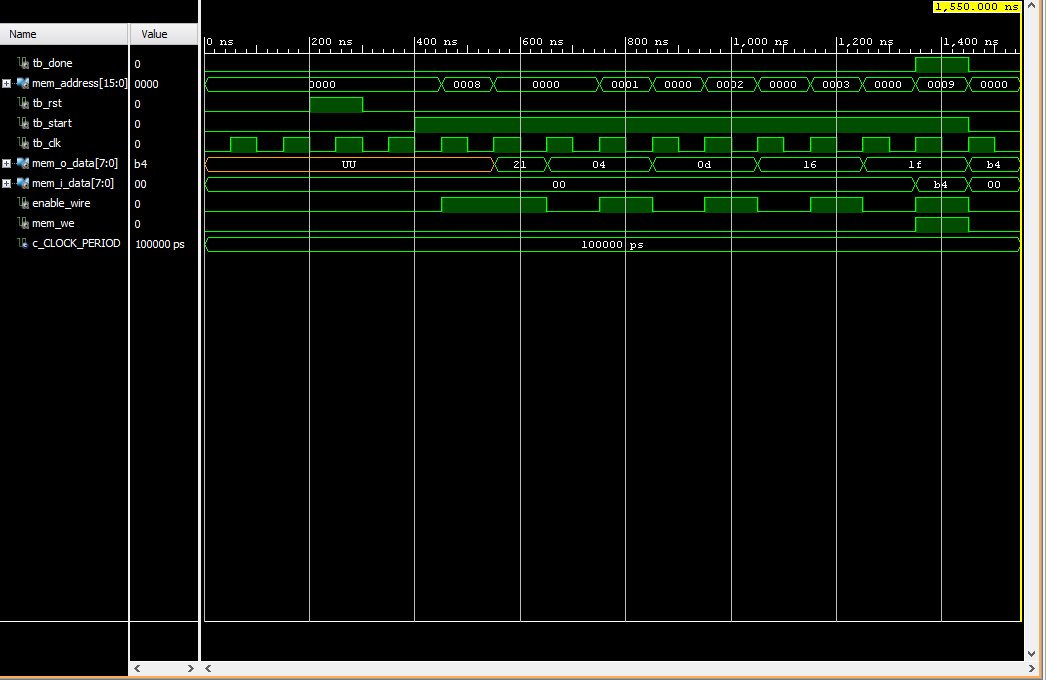
\includegraphics[scale=0.45]{in_wz.png}
        \caption{tb\_pfrl\_2020\_in\_wz}
        \vspace{0.2 cm}
        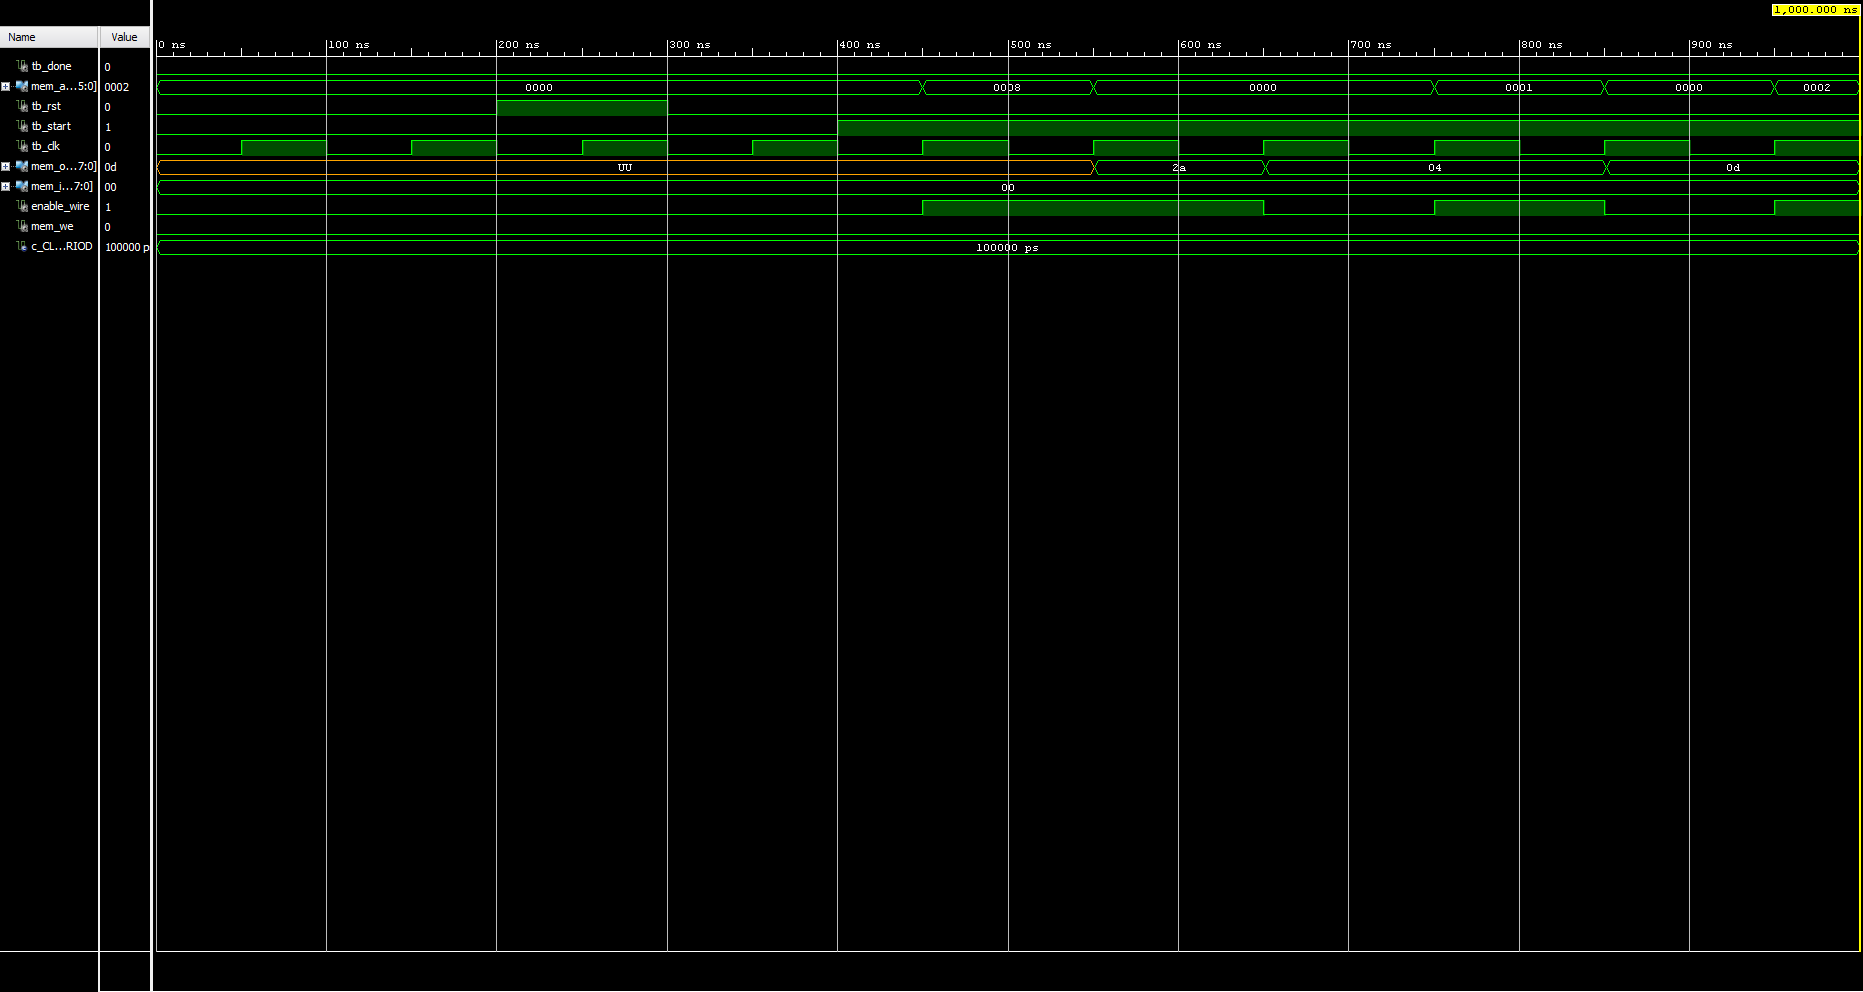
\includegraphics[scale=0.45]{no_wz.png}
        \caption{tb\_pfrl\_2020\_no\_wz}
    \end{center}
\end{figure}
\begin{landscape}
    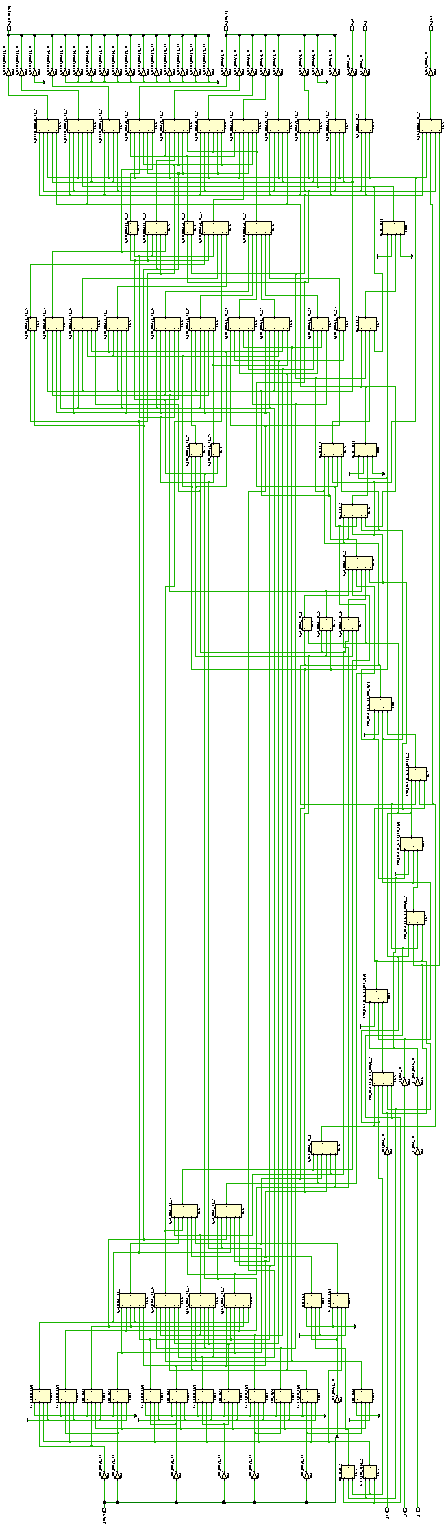
\includepdf[landscape=true, angle= -90,pagecommand=\subsection{Schematic}\thispagestyle{lscape}]{schematic.pdf}
\end{landscape}
\section{Test Benches}
\subsection{\textbf{tb\_pfrl\_2020\_in\_wz}}
In questo test bench si vuole verificare la correttezza del progetto nel caso di un valore appartenente a una working zone, in particolare il valore da codificare è 33.
La posizione 3 di memoria ha il valore 31, quindi l'output corretto per passare questo testbench è 1 (WZ\_BIT) \& 011 (WZ\_NUM) \& 0100(OFFSET).
\subsection{\textbf{tb\_pfrl\_2020\_no\_wz}}
Lo scopo di questo test bench è verificare che nel caso di un valore non appartenente a una working zone, l'output risulti corretto.
Poichè il valore da codificare è 42 e la working zone più vicina ad esso è 37, quindi non esiste 0\(\leq\)offset\(\leq\) 3 tale da raggiungere il valore, l'output risulta 0 (WZ\_BIT) \& 0101010 (42).
\subsection{\textbf{tb\_casi\_limite}}
Sono stati testati i casi limite quali:
\begin{itemize}
    \item valore vicino a una working zone per un offset negativo;
    \item valore appartenente alla prima working zone;
    \item valore appartenente all'ultima working zone;
    \item multipli segnali di reset;
    \item attesa di segnale o\_done \(=\) 0.
\end{itemize}
Per tutti questi casi il progetto ha ottenuto risultati positivi.
\section{Conclusioni}
Dai risultati sperimentali e dalla sintesi si può notare che si ha studiato la codifica working zone con offset one-hot nella sua interezza: testando casi limite, superando le due test benches forniteci, sintetizzando il progetto e analizzandone i risultati.
Una possibile ottimizzazione potrebbe essere gestire il valore di o\_data ad ogni stato con un registro apposito per evitare di avere valori undefined, anche quando non ci interessa osservarlo, e quindi abbassare il numero di LUT ed eliminare un inferring latch.
\end{document}